\subsection{Catalog Completeness, Effectiveness, and Reliability}
\label{s:candr}

To evaluate the performance of the Robovetter and to measure the catalog completeness and reliability, we run the Robovetter on the \injtce{s}, \invtce{s}, and \scrtce{s}. As a high level summary, Figure~\ref{f:scoregrid} provides the completeness, effectiveness ($E$), and reliability for a 3 by 3 grid across period and MES. If the same figure is made for only the FGK dwarf type stars (\logg~$\ge$~4.0 and 4000~K~$\ge$~\tstar~$<$~7000~K), the long period, low MES bin improves substantially. Giant stars are inherently noisy on time scales of planet transits \citep[see Figure~9 of][]{Christiansen2012} causing more FPs and also causing more real transits to be distorted by the noise. For FGK dwarf stars and only considering candidates with periods between 200~d and 500~d and MES~<~10, $C=76.7\%$, $1-E=1.1\%$, and $R=50.3\%$, which is a 13.1 percentage point improvement in reliability and 3 percentage point improvement in completeness compared to all stars in the same period and MES range.

\begin{figure}[hp]
\begin{center}
\begin{tabular}{c}
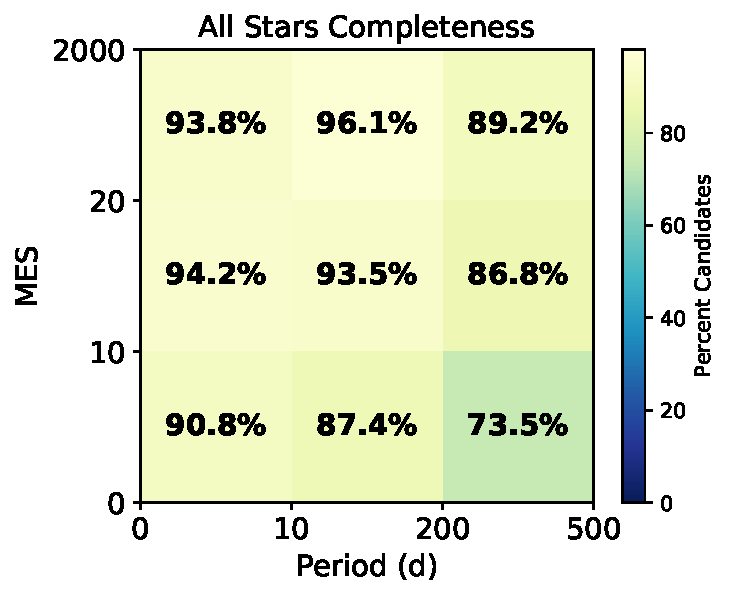
\includegraphics[width=0.92\linewidth]{f8-top.pdf} \\
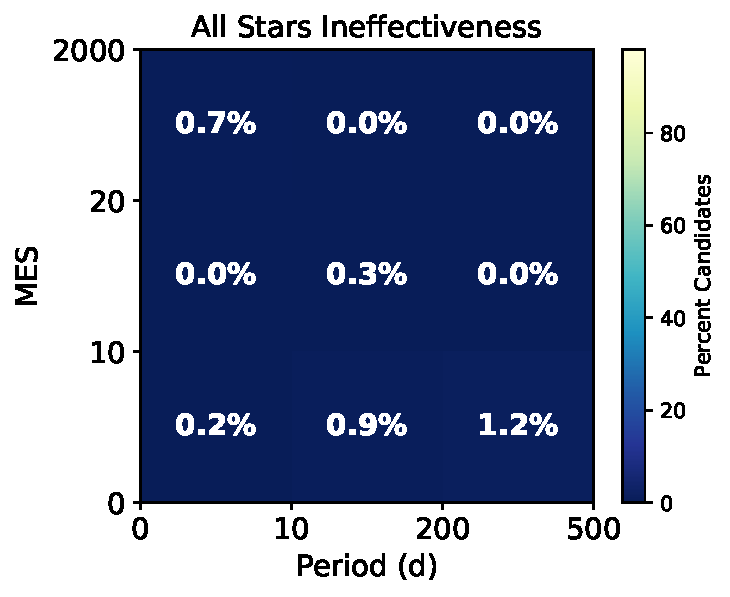
\includegraphics[width=0.92\linewidth]{f8-middle.pdf} \\
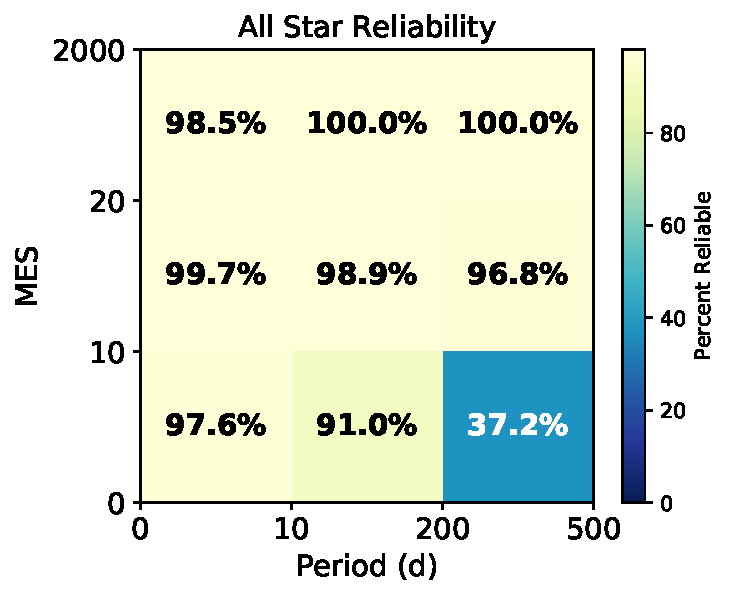
\includegraphics[width=0.92\linewidth]{f8-bottom.pdf}
\end{tabular}
%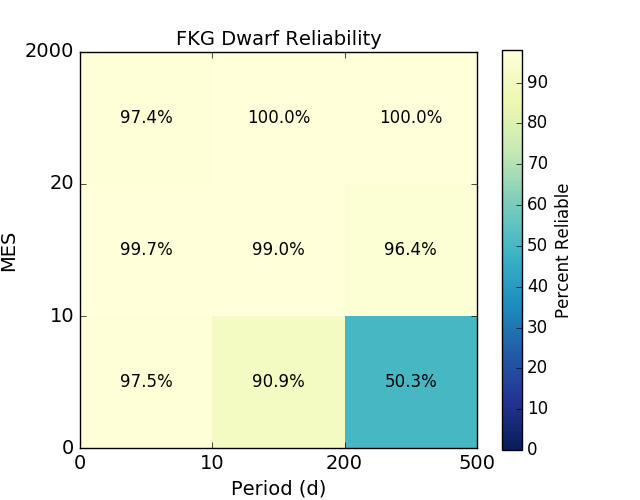
\includegraphics[width=0.48\linewidth]{fig-FgkReliabilityPmes.png}
%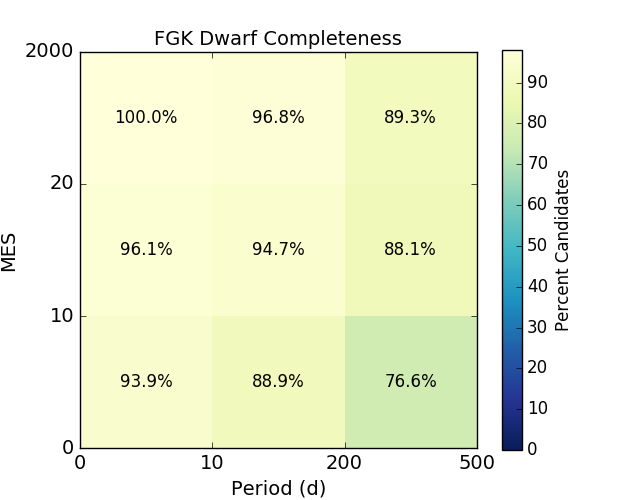
\includegraphics[width=0.48\linewidth]{fig-FgkCompletePmes.png}
\caption{A coarse binning of the completeness, effectiveness, and reliability for different period and MES bins (shown from top to bottom, respectively). \added{(The number of TCEs in the box is shown below the percentage for completeness and effectiveness. The number of PCs is given below the reliability.)}The effectiveness and reliability are based on the combined \invtce{} and \scrtce{} data sets. Notice that the Robovetter effectiveness at removing these false alarms is incredibly high, but for long periods and low MES the resulting reliability is lower because of the large number of false alarms and small number of true planets. For FGK dwarf stars only, the reliability is 50.3\%,\added{ the effectiveness is 98.9\%, and }the completeness is 76.7\% for planets in the longest period, lowest MES box. }
\label{f:scoregrid}
\end{center}
\end{figure}


%For the later, we use the parameters provided by the supplemental DV fits.  \citet{Christiansen2017} shows that the radii based on the MCMC fits match those of the supplemental DV fits. We do not provided MCMC fits of the entire set of false positives in the \opstce\ set and so cannot use them for our analysis here.

\subsubsection{Completeness}
\label{s:comp}
The completeness of the vetting is measured as the fraction of \injtce{s} that are dispositioned as PCs. We discuss here the detection efficiency of the Robovetter, not the Kepler Pipeline (see \S\ref{s:occurates} for a discussion of the Pipeline completeness). Across the entire set of recovered \injtce{s} which have periods ranging from 0.5--500\,d, the Robovetter dispositioned \completeness{}\% as PC. As expected, the vetting completeness is higher for transits at shorter periods and higher MES, and lower for longer periods and lower MES. The right hand column of Figure~\ref{f:1dcompare} shows how the completeness varies with period, expected MES, number of transits, and transit duration. Note that expected MES is the average MES at which the injected transit signal would be measured in the target light curve, given the average photometric noise of that light curve and the depth of the injected transit signal --- see \citealt{Christiansen2017} for more details. The small drop in completeness just short of 90\,days is likely caused by the odd-even metric (\S\ref{s:oddeven}), which only operates out to 90\,days, confusing true transits for binary eclipses.  


\begin{figure*}[hp]
 \begin{center}
  %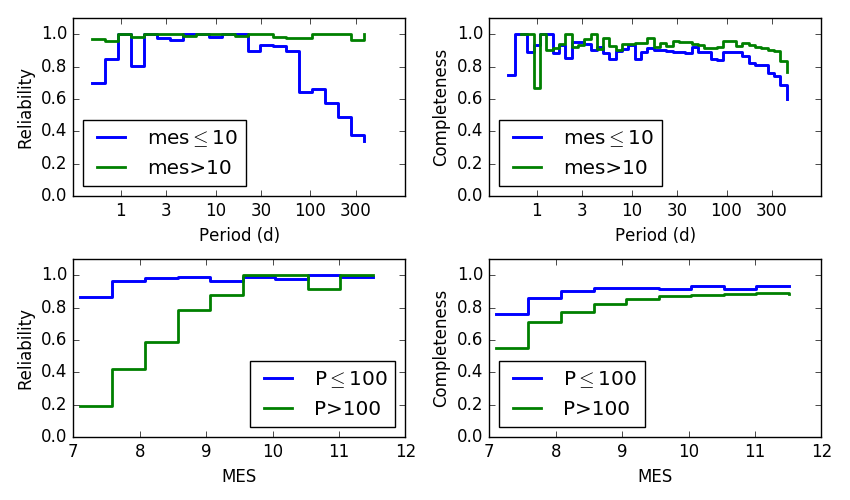
\includegraphics[width=0.9\linewidth]{fig-compRel1D-PerMes.png}
  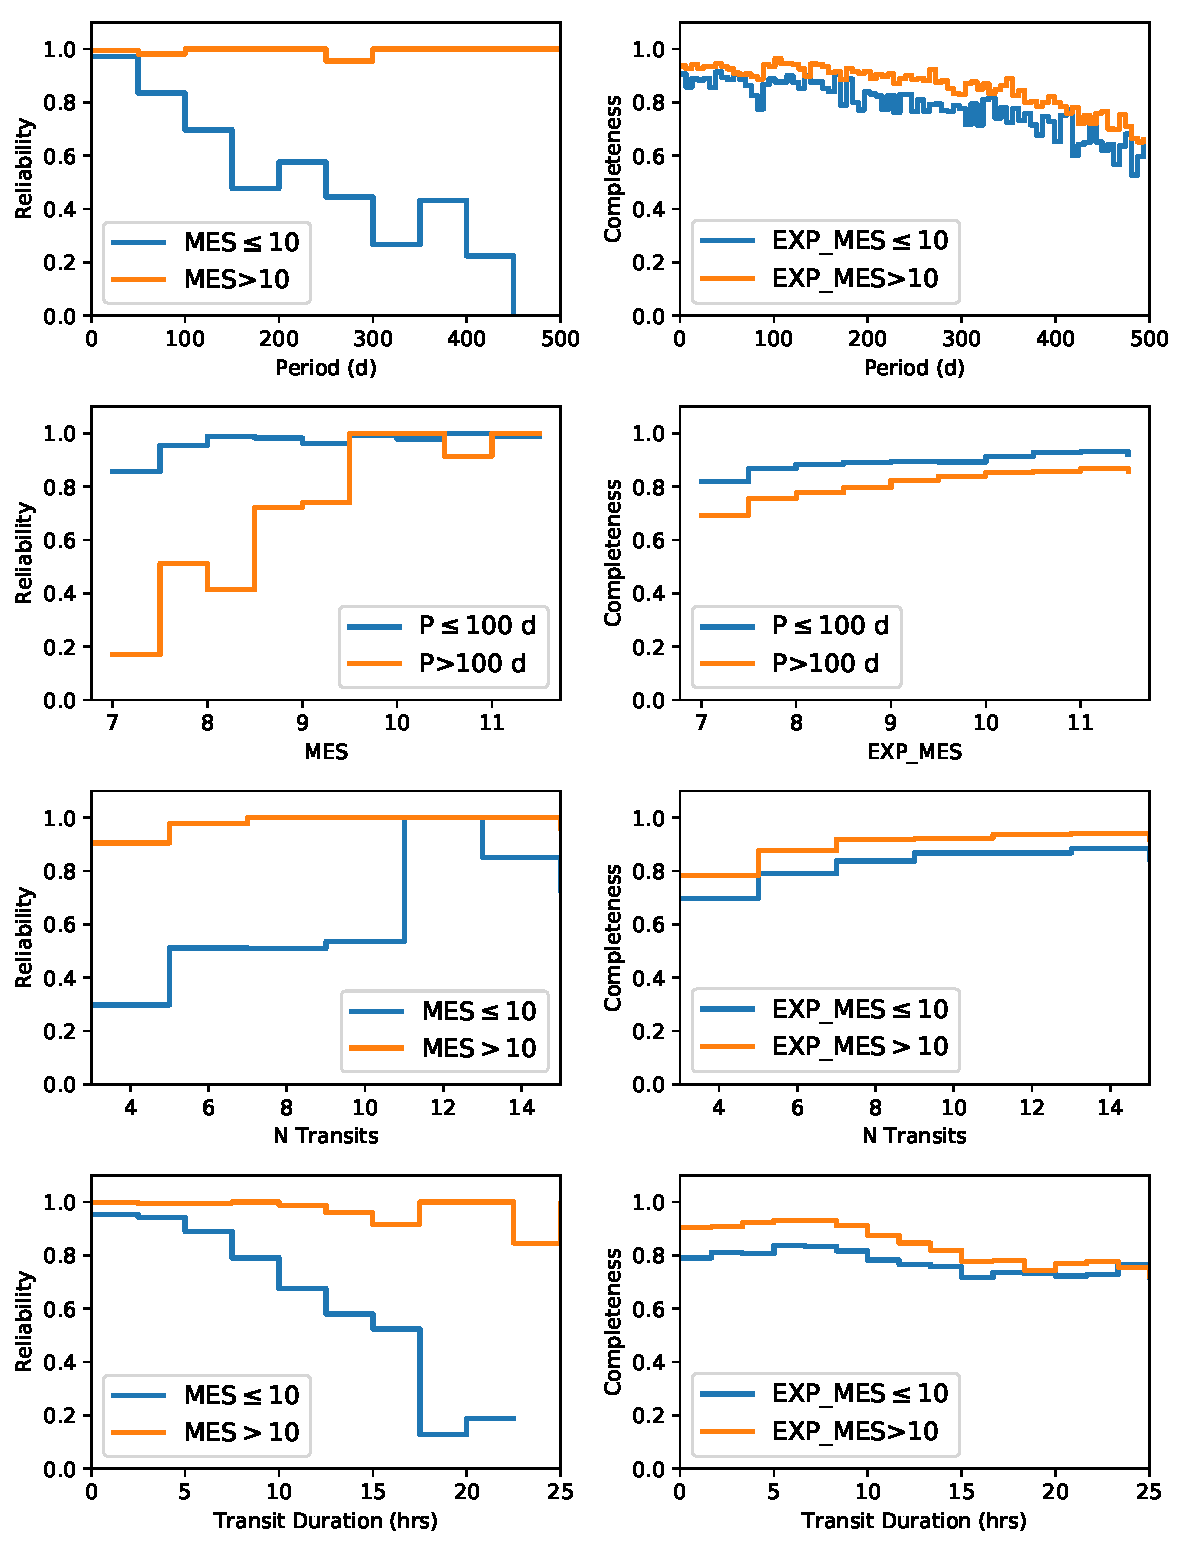
\includegraphics[width=0.875\linewidth]{f9.pdf}
  \caption{The reliability (left) and completeness (right)  of the DR25 catalog plotted as a function of period, MES, number of transits, and transit duration. In each case the blue line is for those with MES~$\leq$~10 or periods~$\leq$~100\,d. The orange line shows the completeness or reliability for the rest of the population (see the legend for each plot). EXP\_MES is the expected MES (see \citealt{Christiansen2017} and \S\ref{s:comp}).}
  \label{f:1dcompare}
 \end{center}
 \end{figure*}


Because most planet occurrence rate calculations are performed using period and radius \citep[e.g.,][]{Burke2015}, we show the measured completeness binned by period and radius in Figure~\ref{f:prCompleteness}. The plot is linear in period and radius in order to emphasize the long period planets. Planetary radius is not a natural unit to understand the performance of the Robovetter since it combines the depth of the transit, the noise level of the light curve, and the stellar radius.  At the longest periods the Robovetter more often fails the largest planets, though the trend is reduced when only considering the FGK dwarf stars. The largest radii planets in the \injtce{} population are entirely around giant stars, because large planets were not injected onto the dwarf stars \citep{Christiansen2017}. The giant stars are notoriously noisy. As a result the largest radii planets in the \injtce{s} are more likely to be dispositioned incorrectly. Also, even when only considering the dwarf stars, a larger fraction of the big planets will be around larger, more massive stars (in comparison to the small planets which will mostly be found around smaller stars). This results in a population of planets that produce longer transit durations. The Robovetter performs less well for long transit durations (see Figure~\ref{f:1dcompare}). For more figures showing the Robovetter effectiveness across different parameters, see \citet{Coughlin2017a}.
%For example, the probability of a planet's single transit overlapping a cadence impacted by image artifacts is higher (\S\ref{s:skye}) or the fit performed by Mars 


\subsubsection{Effectiveness}
The effectiveness of the Robovetter at identifying instrumental and stellar noise is calculated using the union of the \invtce{s} and \scrtce{s} (see \S\ref{s:relcalc}), after removing the TCEs specified in \S\ref{s:clean}. Across the entire set, the Robovetter dispositions 99.6\% of these simulated false alarms as FPs.  Only 119 of the 28,735 simulated false alarms are dispositioned as a PC by the Robovetter.  Most of these invPCs and scrPCs are at long periods and low MES. However, using the 4544 \invtce s and \scrtce s that have periods between 200\,d and 500\,d and MES less than 10, the Robovetter's effectiveness is 98.8\% (see Figure~\ref{f:scoregrid}).  Unfortunately, because there are so few candidates at these long periods, this translates to a relatively low reliability.  For detailed plots showing how effectiveness varies with different parameters see \citet{Coughlin2017a}.


\subsubsection{Reliability}
\label{s:reliability}
The reliability is measured according to the method described in \S\ref{s:relcalc} using the effectiveness measured from the combined \scrtce{} and \invtce{} data sets and the number of observed PCs.  If one bins over the entire data set, the overall reliability of the catalog is 97\%. However, as Figure~\ref{f:1dcompare} demonstrates, the reliability for long period, and especially low MES planets, is significantly smaller.  For periods longer than 200\,d and MES less than 10, the reliability of the catalog is approximately 37\%, i.e., 6 out of 10 PCs are caused by noise. As with completeness, we plot the reliability as a function of period and planet radius in Figure~\ref{f:prReliability}. The least reliable planets are at long periods and have radii less than 4\re. 


\begin{figure*}[ht]
\begin{center}
\begin{tabular}{cc}
%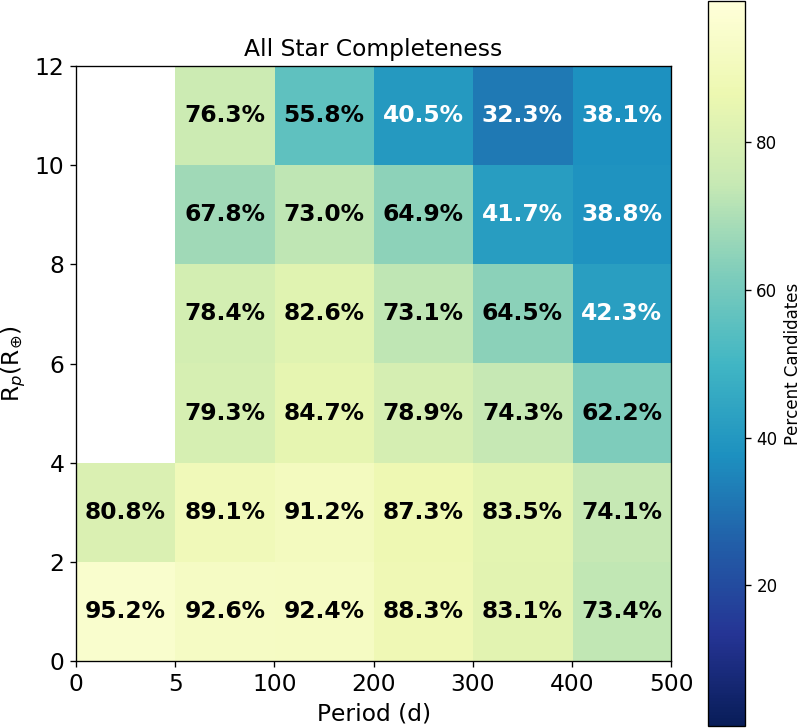
\includegraphics[width=0.5\linewidth]{fig-AllCompletePR-trimmed.png} &
%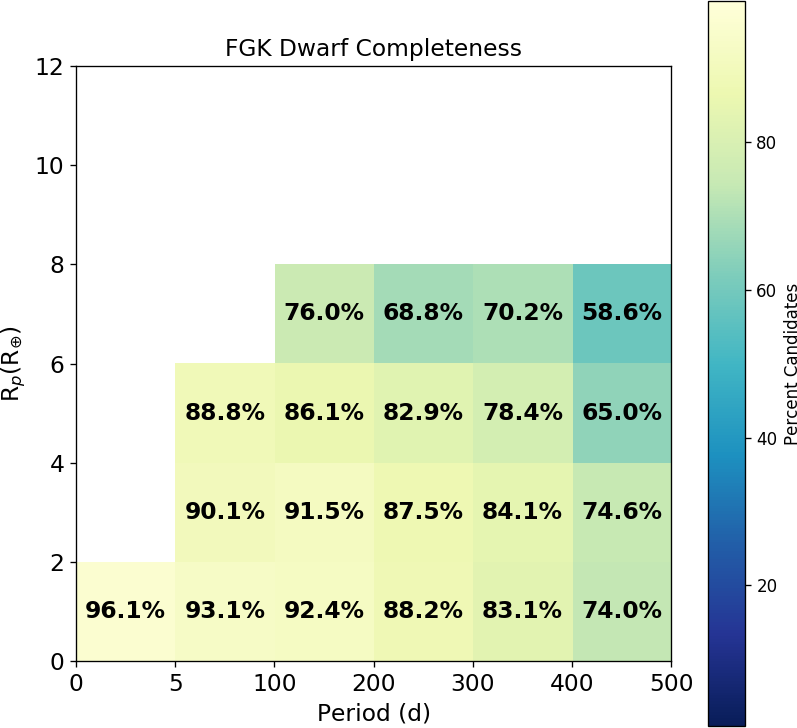
\includegraphics[width=0.5\linewidth]{fig-FgkCompletePR-trimmed.png}
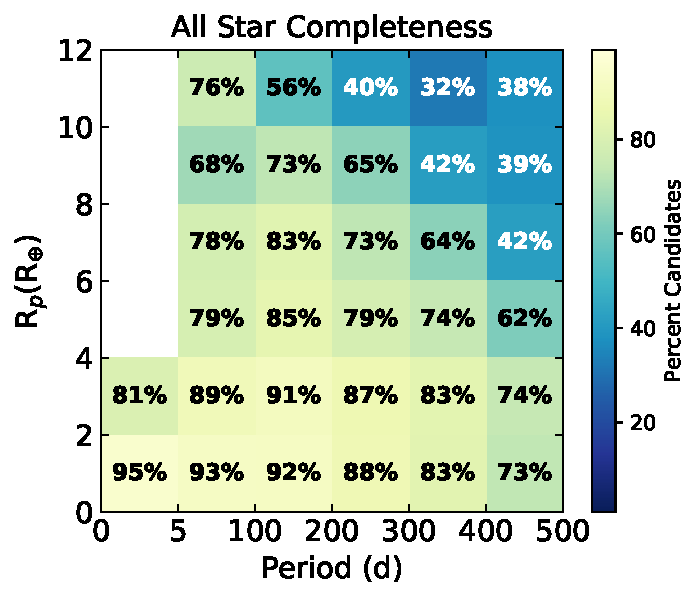
\includegraphics[width=0.5\linewidth]{f10-left.pdf} &
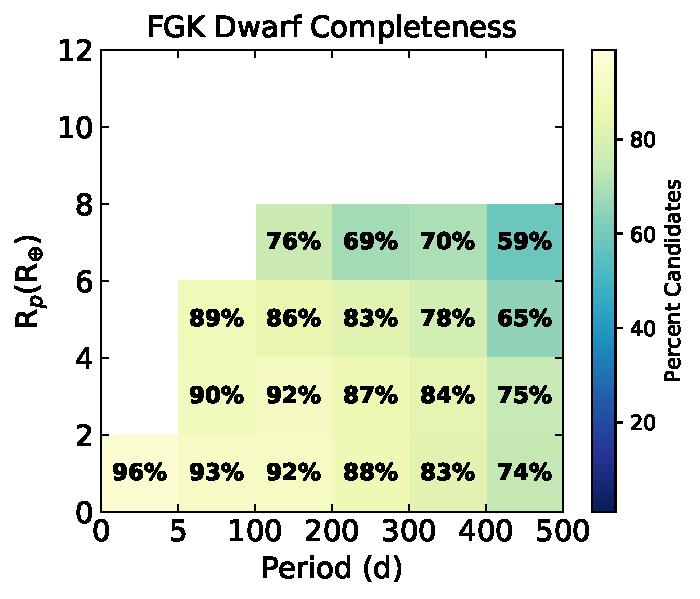
\includegraphics[width=0.5\linewidth]{f10-right.pdf}
\end{tabular}
\caption{The Robovetter completeness binned by period and planet radius for all stars (left) and for only FGK dwarf stars (right). Bins with fewer than 10 \injtce{s} are not plotted.}
\label{f:prCompleteness}
\end{center}
\end{figure*}


\begin{figure*}[htb]
\begin{center}
\begin{tabular}{cc}
%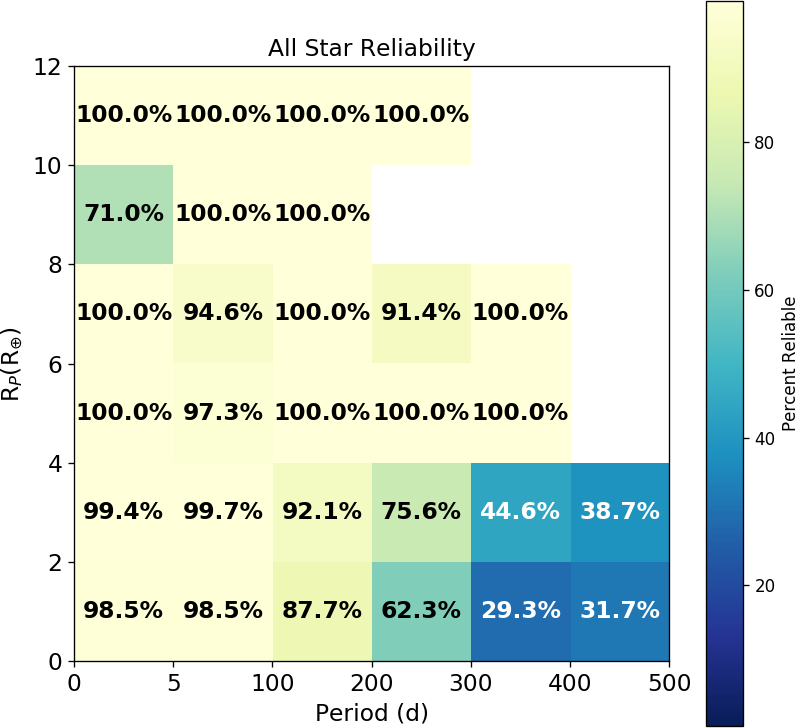
\includegraphics[width=0.5\linewidth]{fig-AllReliabilityPR-trimmed.png} &
%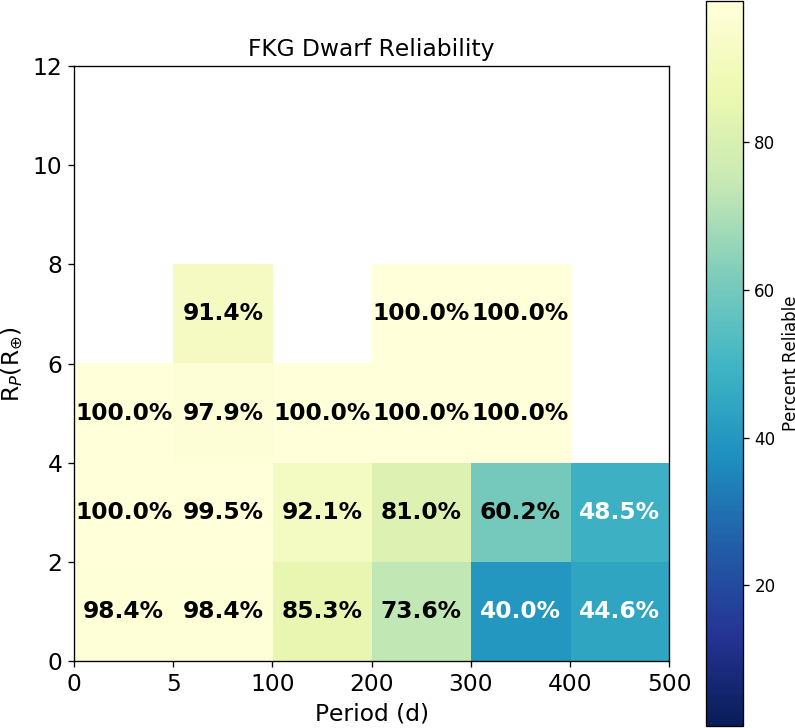
\includegraphics[width=0.5\linewidth]{fig-FgkReliabilityPR-trimmed.png}
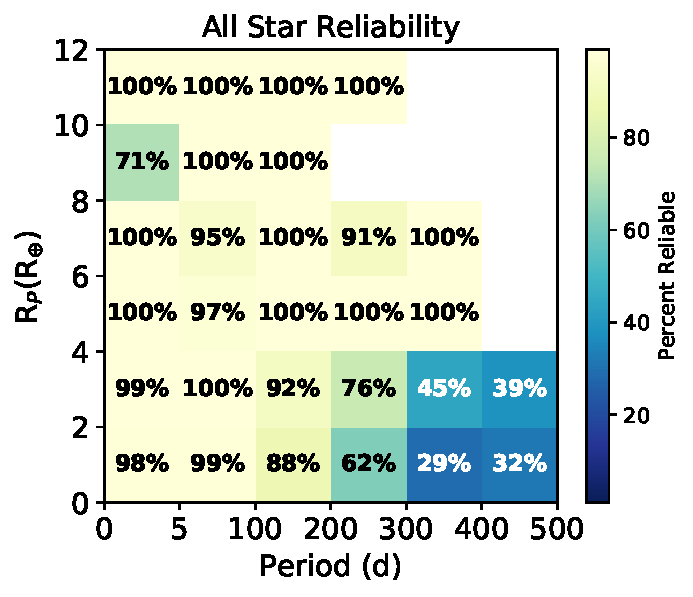
\includegraphics[width=0.5\linewidth]{f11-left.pdf} &
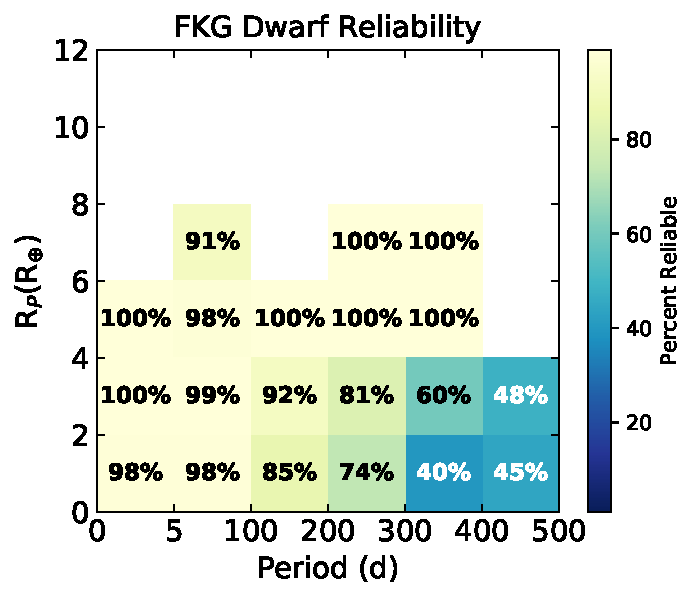
\includegraphics[width=0.5\linewidth]{f11-right.pdf}
\end{tabular}
\caption{A 2D binning of the candidate catalog reliability for period and planet radius for all stars (left) and for the FGK dwarf stars (right). Bins with fewer than 3 candidates or fewer than 20 simulated false alarms (from \invtce{} and \scrtce{}) are not plotted.}
\label{f:prReliability}
\end{center}
\end{figure*}


The uncertainty in the reliability is likely dominated by how well the false alarms in the \scrtce{} and \invtce{} sets match the false alarms in the \opstce{} data set (see \S\ref{s:simularity} for further discussion on their similarity).  One way to get a handle on the uncertainty on reliability is to calculate the reliability in three different ways for the long period (200--500\,d), low MES ($<10$) \opstce{s}.  First, we use only the \invtce{s} to measure the effectiveness at removing false alarms. This results in a lower reliability, namely $R$~=~24\% with $E$~=~98.5\%. Second, we use only the \scrtce{s} to measure the effectiveness. This results in a higher reliability, $R$~=~51\% with $E$~=~99.1\%. Third, we select, at random, half of the combined population of false alarms (\scrtce{} and \invtce{}) and calculate the reliability. After doing this random selection 100 times, we obtained $R$~=~38\% with a standard deviation of 8\%, and the distribution appears symmetric and basically Gaussian in shape.  

The Robovetter is less effective at removing the false alarms produced by inversion than those by scrambling the data. Inversion finds false alarms with periods near 372\,d, which are frequently caused by image artifacts.  Scrambling under-populates these types of false alarms, and since they are the difficult to eliminate, it is not surprising that the reliability measured by inversion is worse than scrambling.  The truth likely lies somewhere in between. We encourage users of these data sets to consider ways to optimize the reliability measurement, and the error budget associated with them, when doing occurrence rate calculations. 




\subsubsection{High Reliability Using the Disposition Score}
\label{s:crscores}

The disposition scores discussed in \S\ref{s:scores} can be used to select a more reliable, though more incomplete, sample of planet candidates. In Figure~\ref{score-fig-2} we show the distribution of disposition scores for the PCs and FPs from the observed, inverted, scrambled, and on-target planet injection populations. (Note, the inverted and scrambled populations have been cleaned as discussed in \S\ref{s:clean}). For all populations, the PC distribution tends to cluster near a score of 1.0 with a tail that extends towards lower score values. Lower MES values tend to have a greater proportion of lower score values. Similarly, the vast majority of FPs have a score of 0.0, with only a small fraction extending towards higher score values (note the y-axis for the FPs is logarithmic, while the y-axis for PCs is linear). Comparing the populations, the on-target planet injections have a greater concentration of score values towards 0.5 for both the PCs and FPs than other populations. Both the inverted and scrambled populations have very few PCs near high score values. We can exploit the relative distribution of PC and FP score values for the different populations to select a higher reliability catalog.

\begin{figure*}[htb]
\centering
\begin{tabular}{cc}
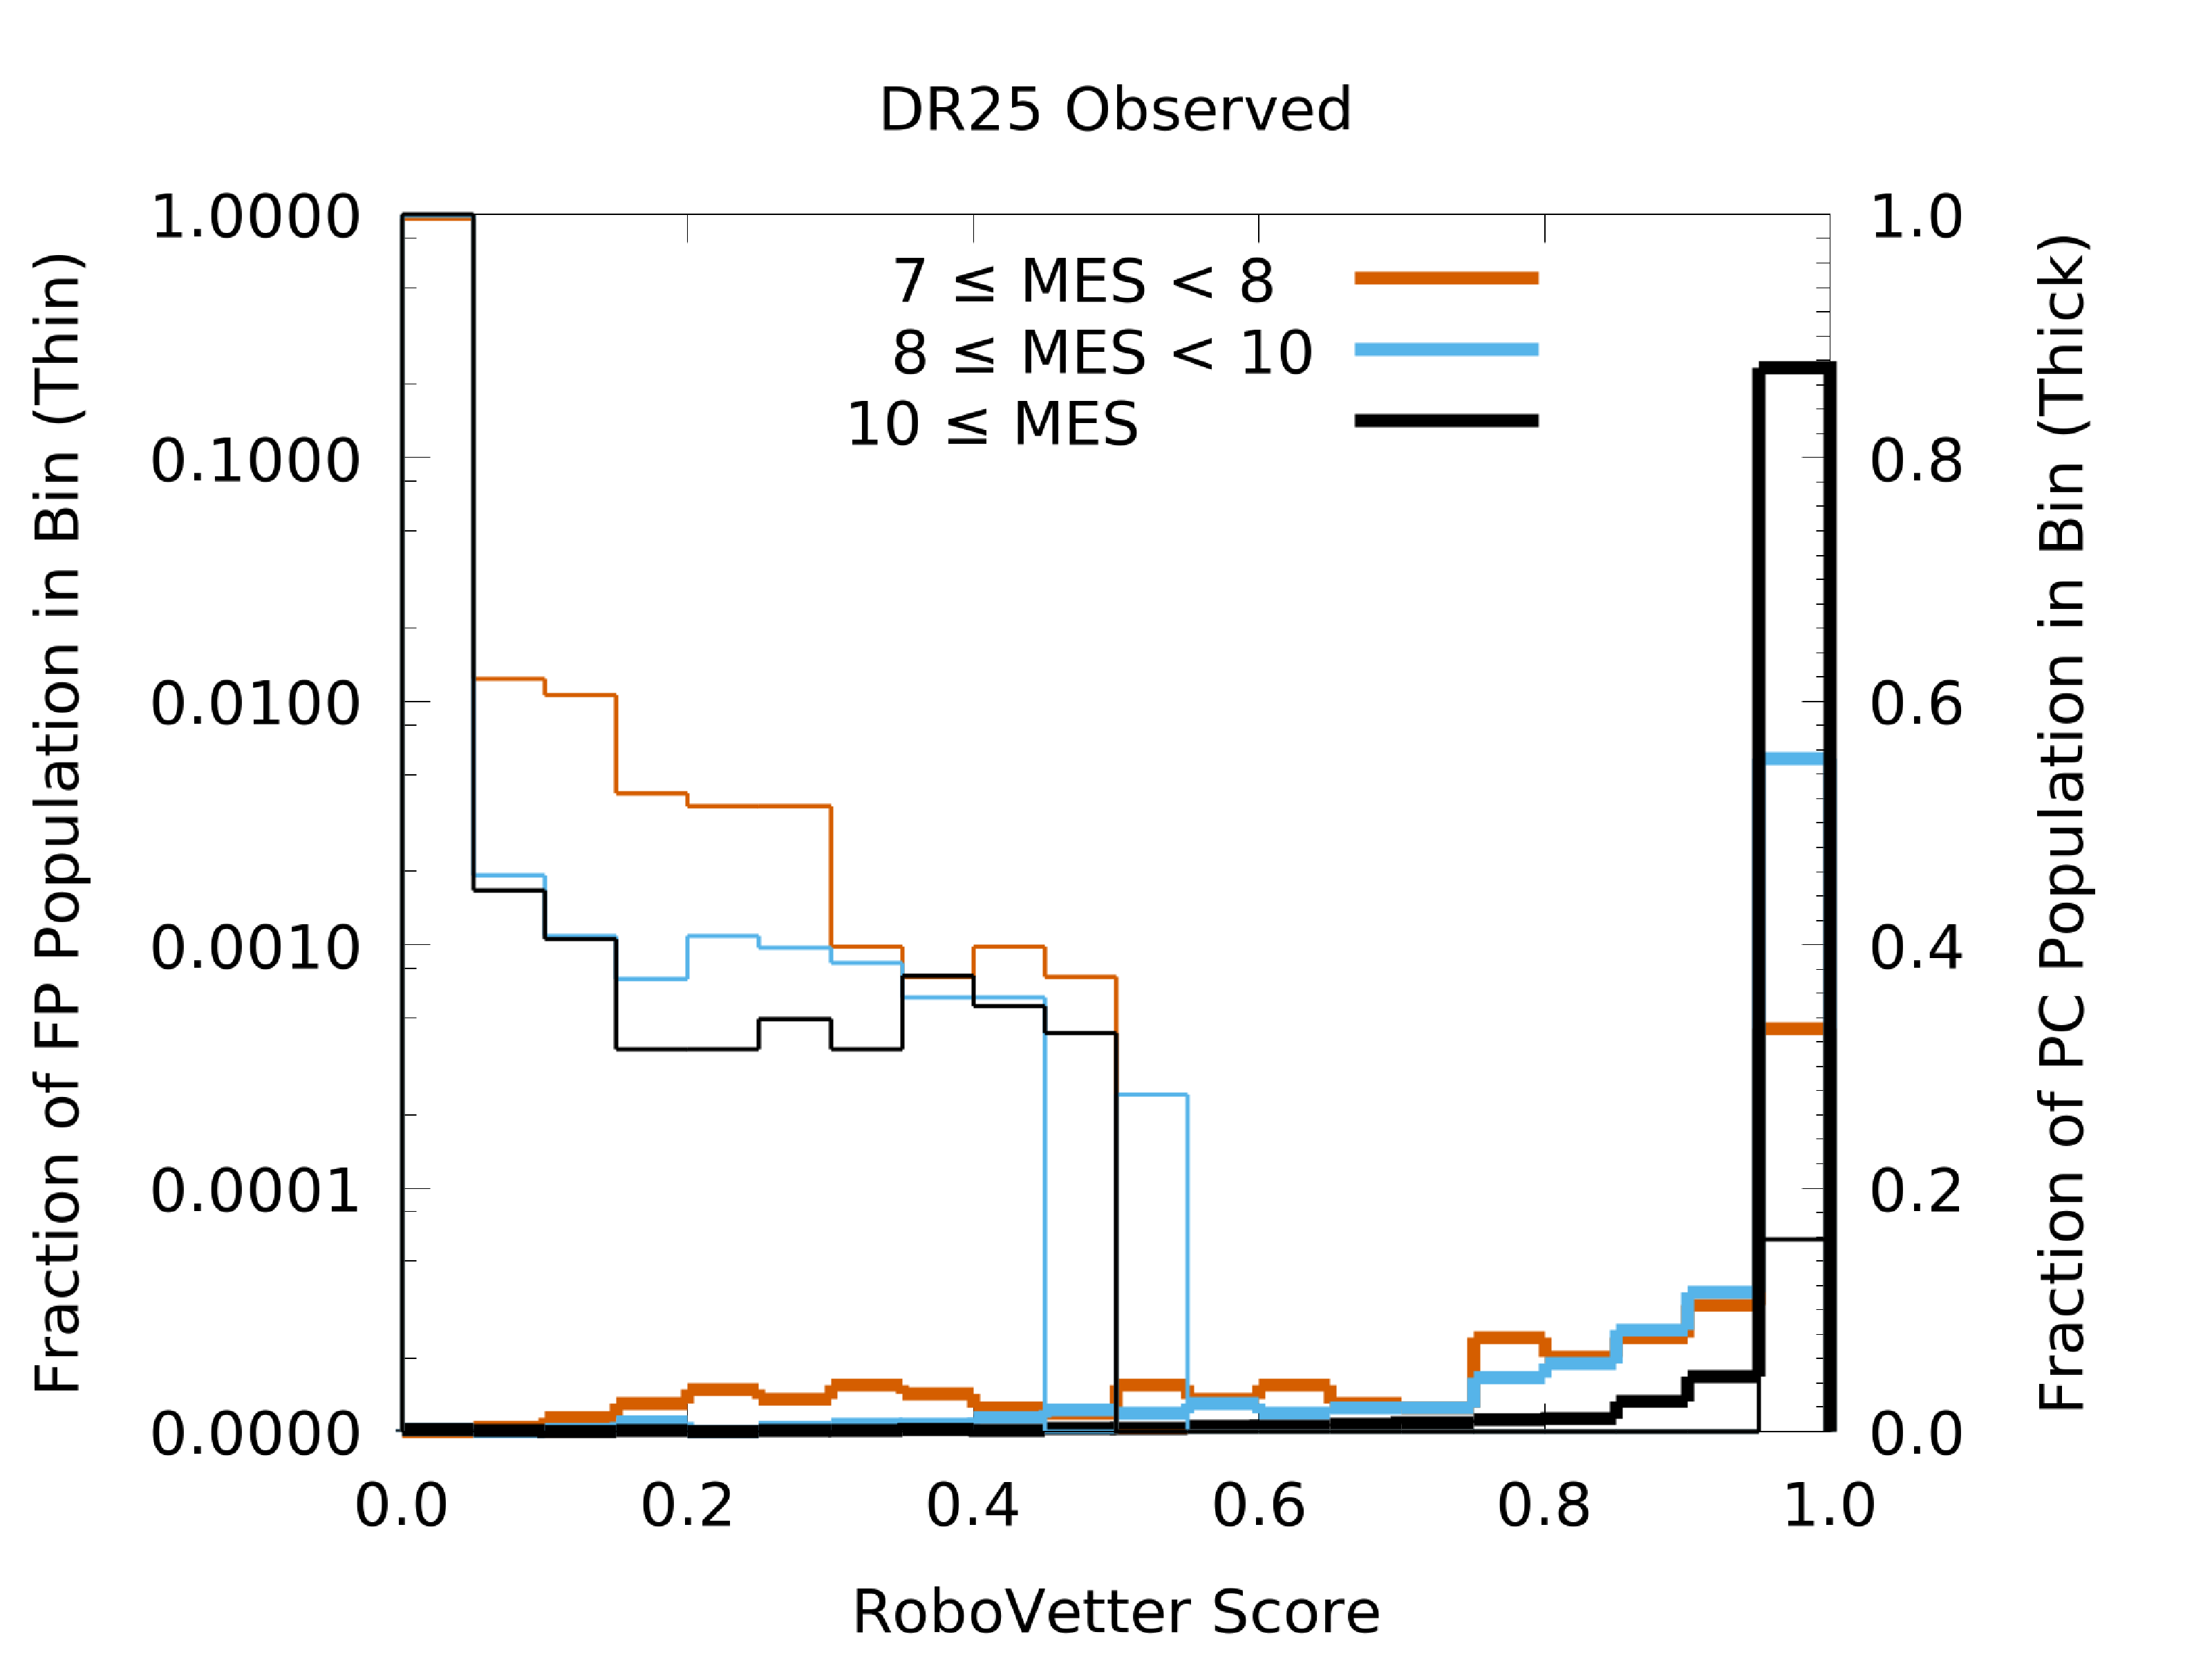
\includegraphics[width=0.5\linewidth]{Scores-OBS.pdf} &
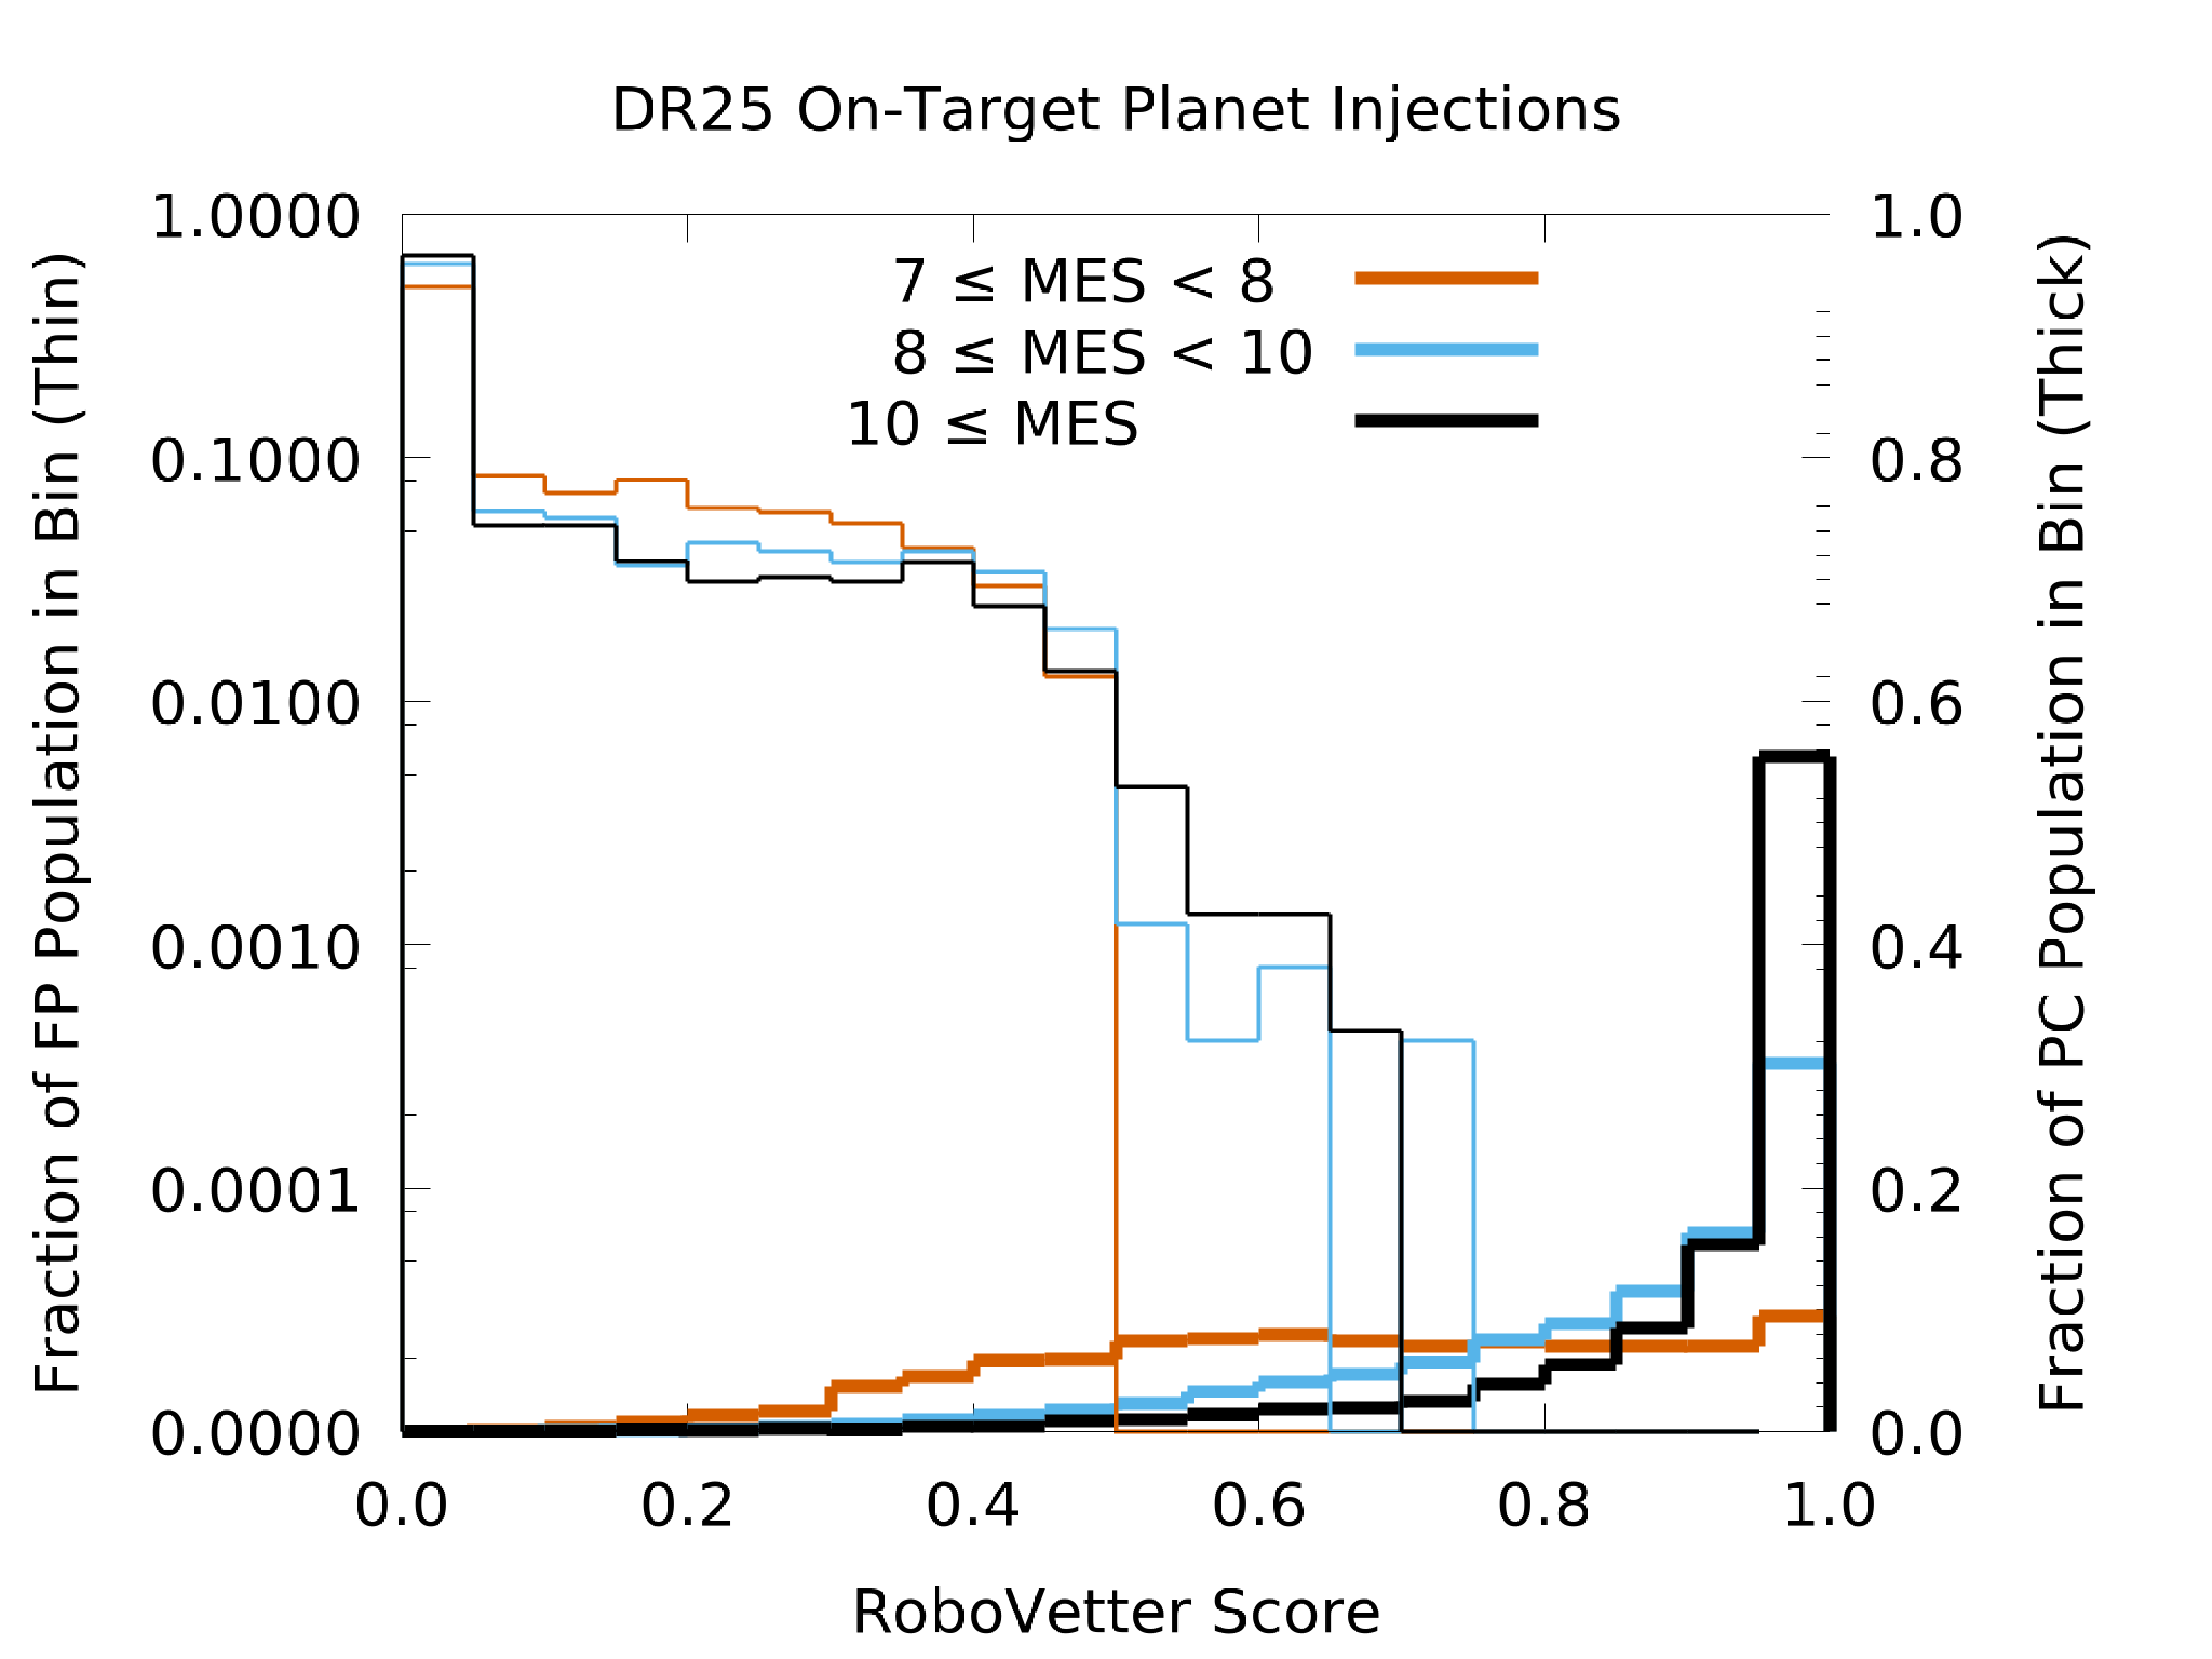
\includegraphics[width=0.5\linewidth]{Scores-INJ1.pdf} \\
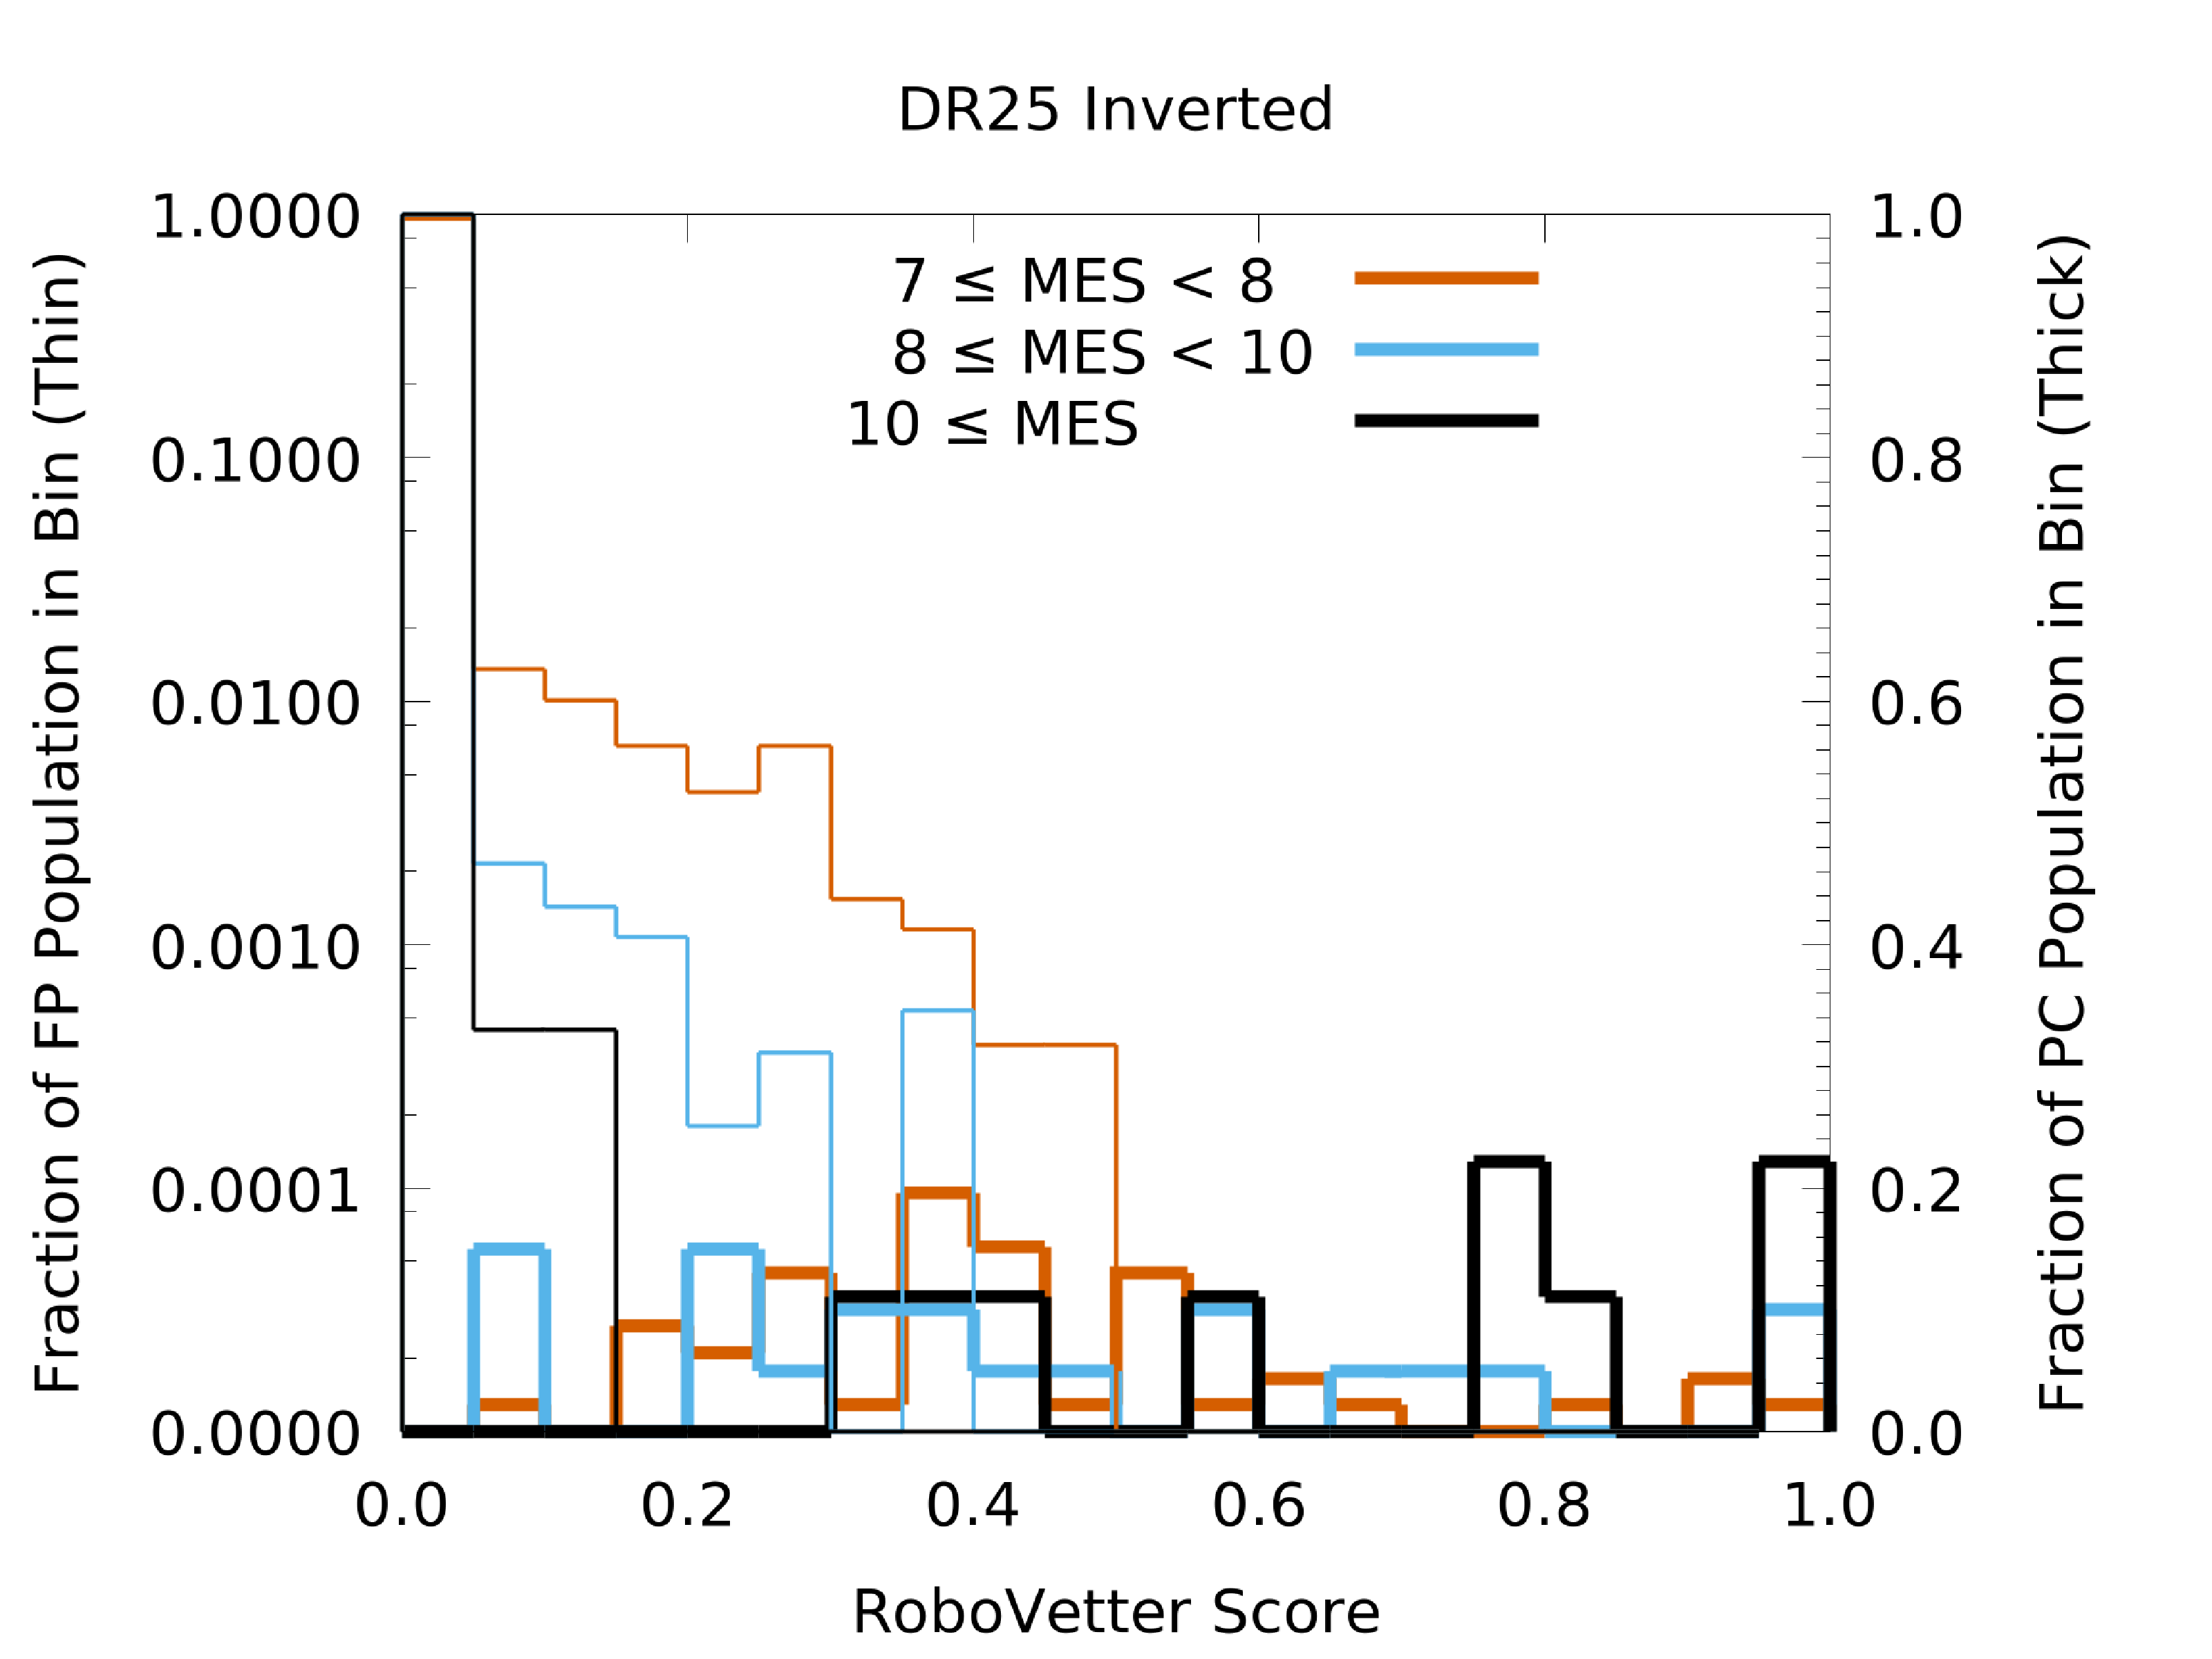
\includegraphics[width=0.5\linewidth]{Scores-INV.pdf} &
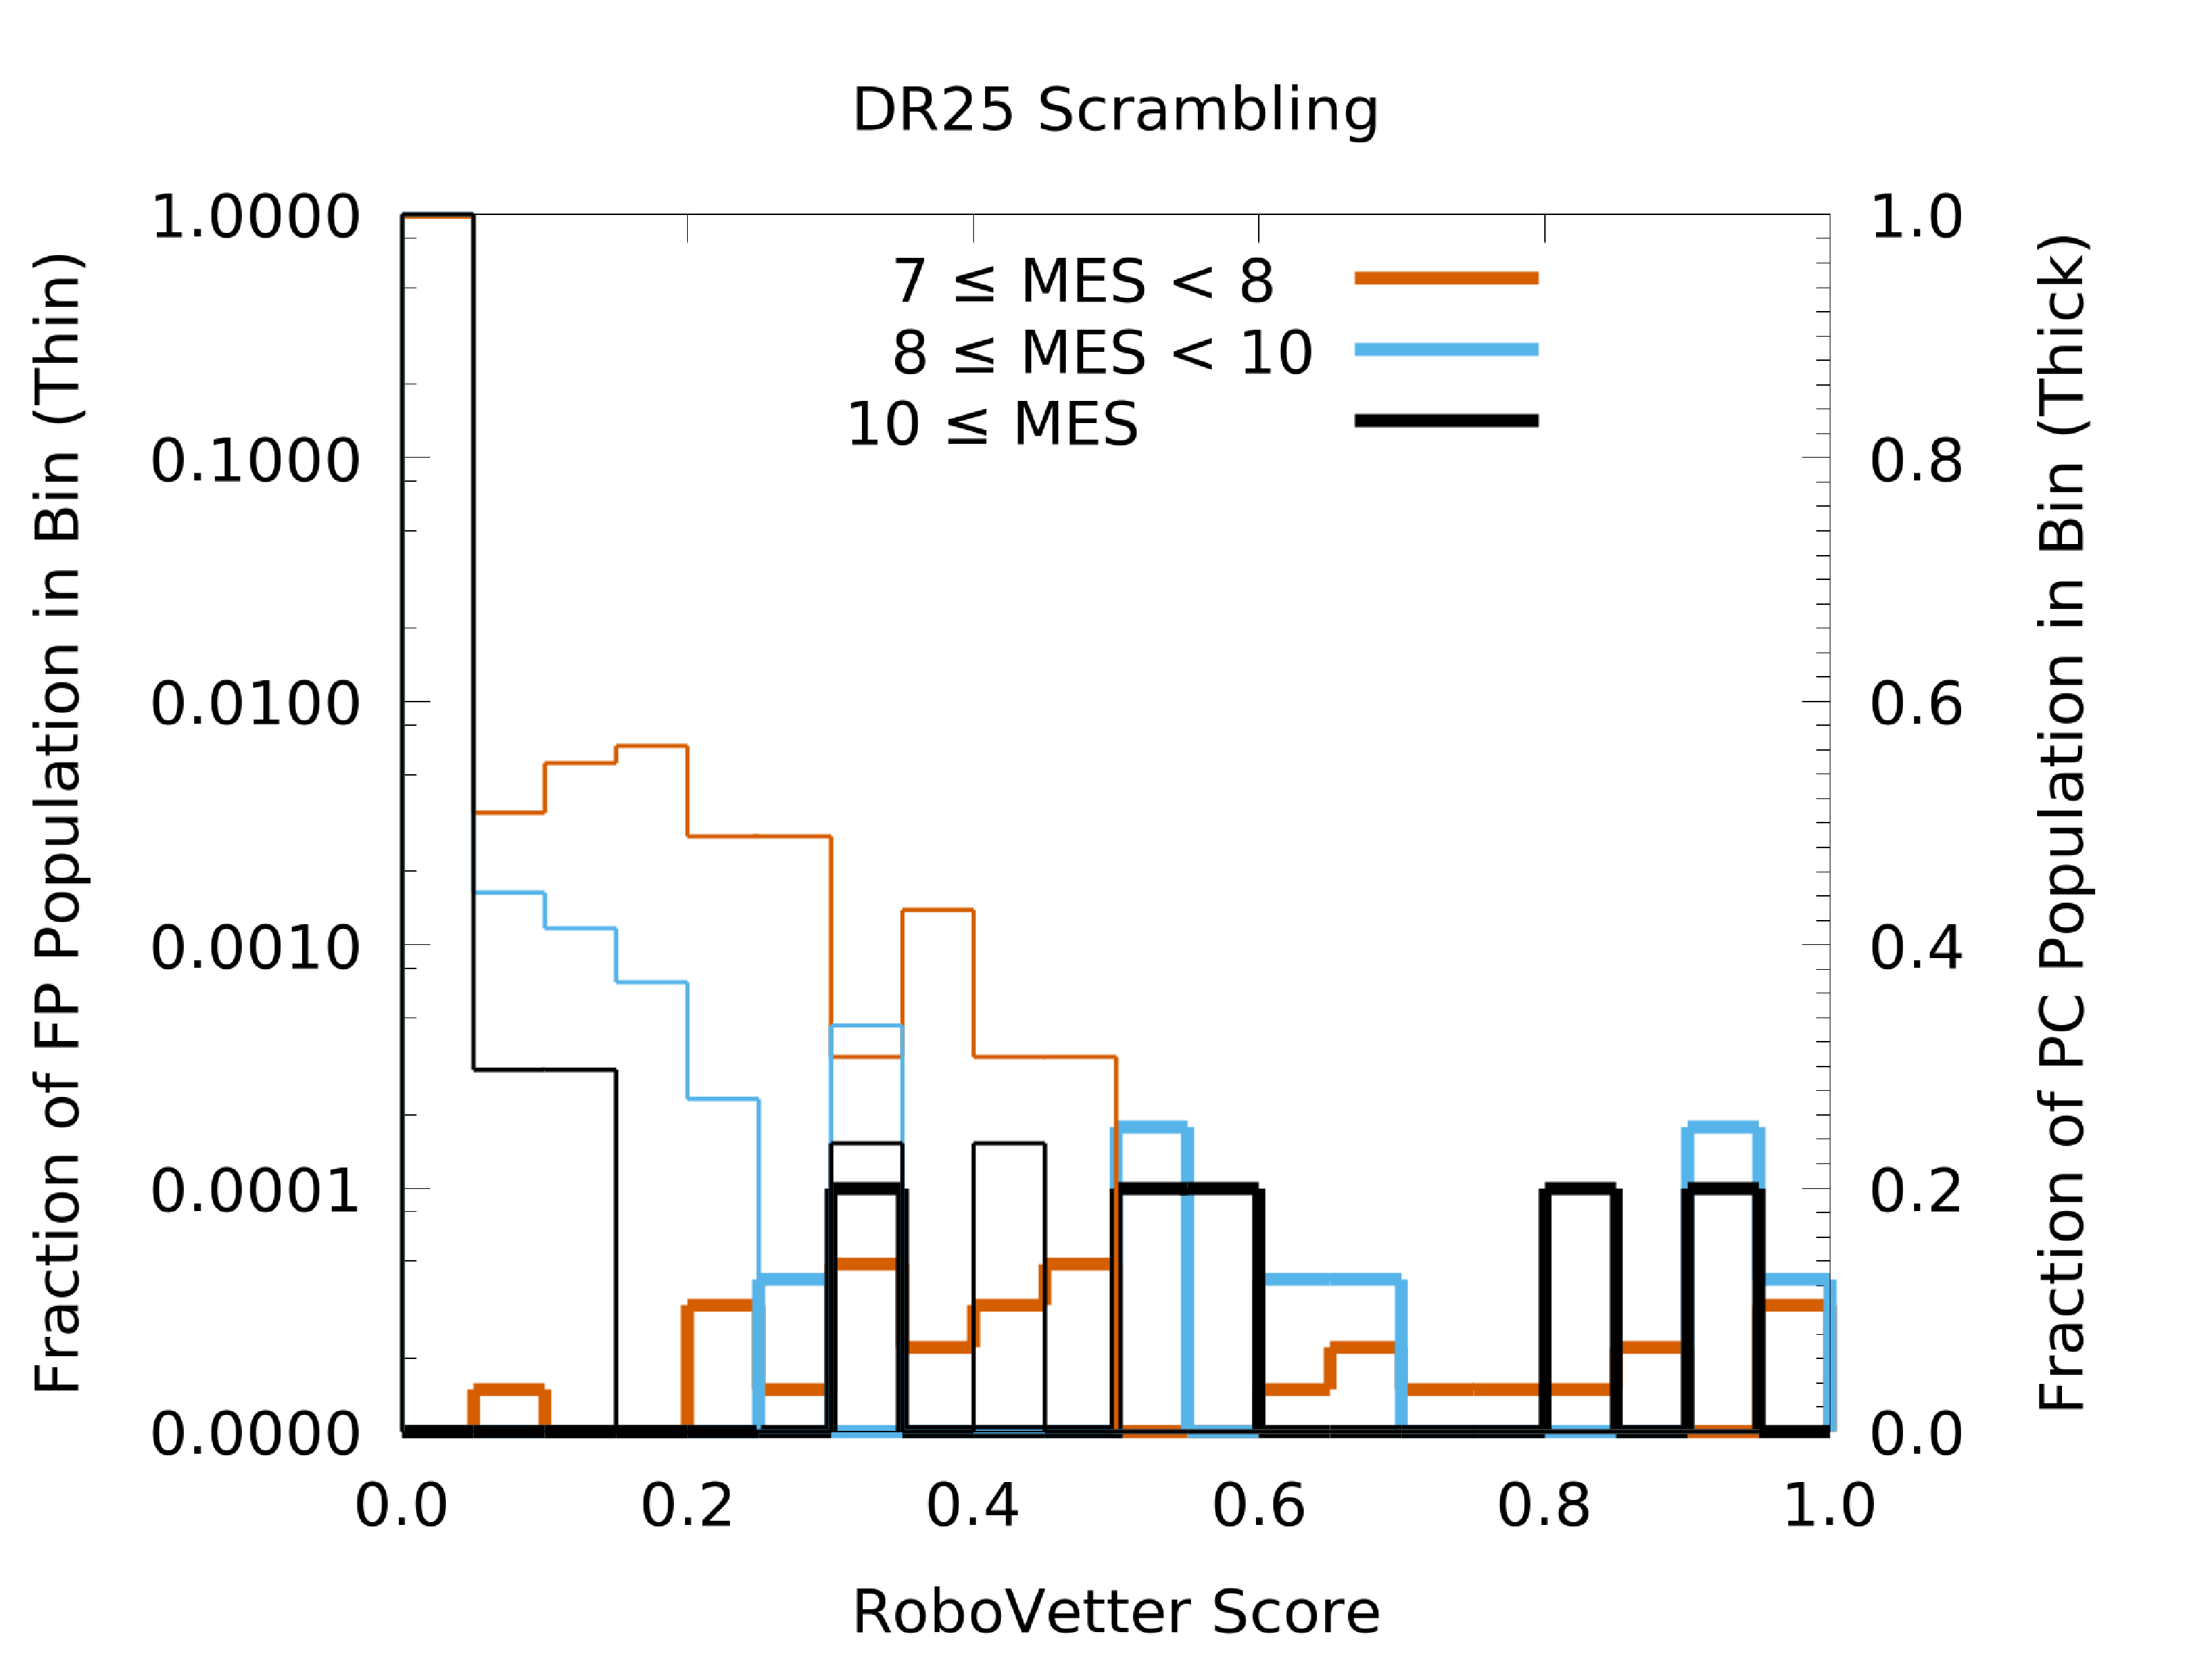
\includegraphics[width=0.5\linewidth]{Scores-SCR1.pdf} \\
\end{tabular}
\caption{Plots of the score distribution of PCs (thick lines, right y-axis) and FPs (thin lines, left y-axis, logarithmic scaling) for the observed (top-left), on-target planet injections (top-right), inverted (bottom-left), and scrambled (bottom-right) TCEs.}
\label{score-fig-2}
\end{figure*}

At the top of Figure~\ref{f:adjscore} we show how the completeness and reliability of the catalog vary for different cuts on the disposition score for MES$<$10 and periods between 200 and 500 days. The effectiveness of the Robovetter increases as the score threshold is increased. The reliability values also depend on the number of observed PCs that remain, which is why reliability does not change in step with the effectiveness. Selecting the PC sample by choosing those with a disposition score above 0.6 (see the point labeled 0.6 on the top of Figure~\ref{f:adjscore}) yields an 85\% reliability and a completeness that is still above 50\%. Doing a score cut in this way not only removes those dispositioned as a PC from the sample, but also causes a few \opstce{s} which are formally dispositioned as FPs to now be included in the sample. An FP with a high score occurs when a TCE marginally fails a single metric.  

It is interesting to note that the number of inferred candidates, i.e., the number of candidates after accounting for the Robovetter completeness and catalog reliability, does not change significantly with the score cut. In the lower plot of Figure~\ref{f:adjscore} we plot both the observed number of PCs and the corrected number of PCs that have periods between 200 and 500 days and MES less than 10.  The correction is done by taking the number of PCs and multiplying by the reliability and dividing by the completeness.  The error bars only include the Poisson counting error in the number of observed PCs and do not include errors in the measured completeness or reliability. The corrected number of PCs only varies by approximately 1$\sigma$ regardless of the score cut used.   

\begin{figure}[htb]
 \begin{center}
 \begin{tabular}{c}
  %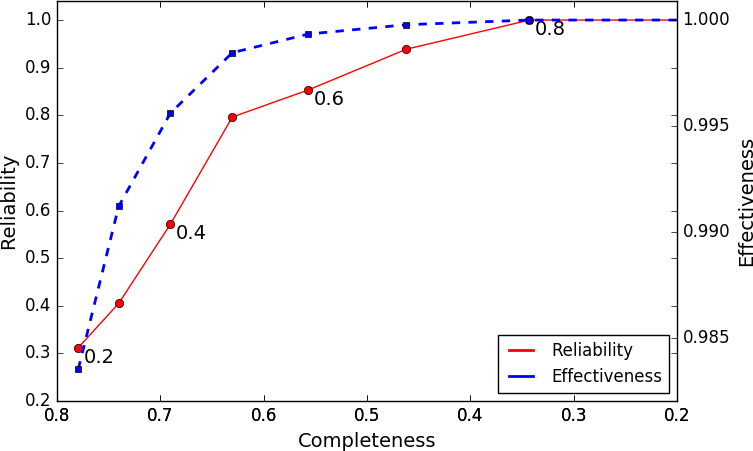
\includegraphics[width=\linewidth]{fig-CRadjustScore-DR25-trimmed.png} \\[12pt]
  %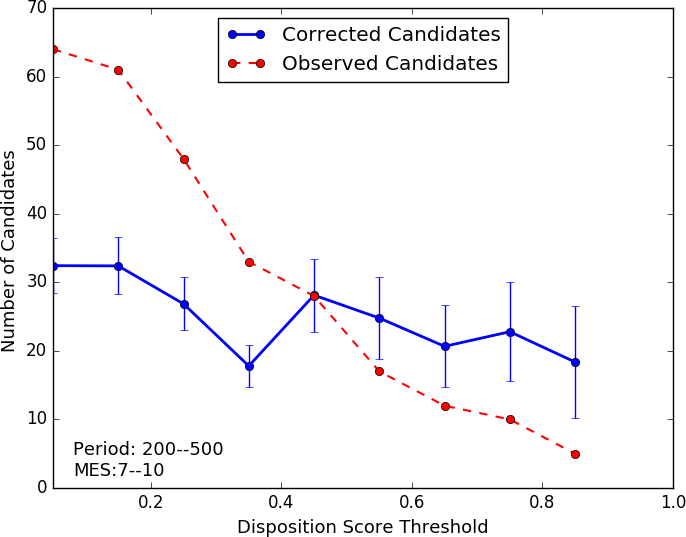
\includegraphics[width=\linewidth]{fig-varyScoreNcandidatesBox2-trimmed.png}
   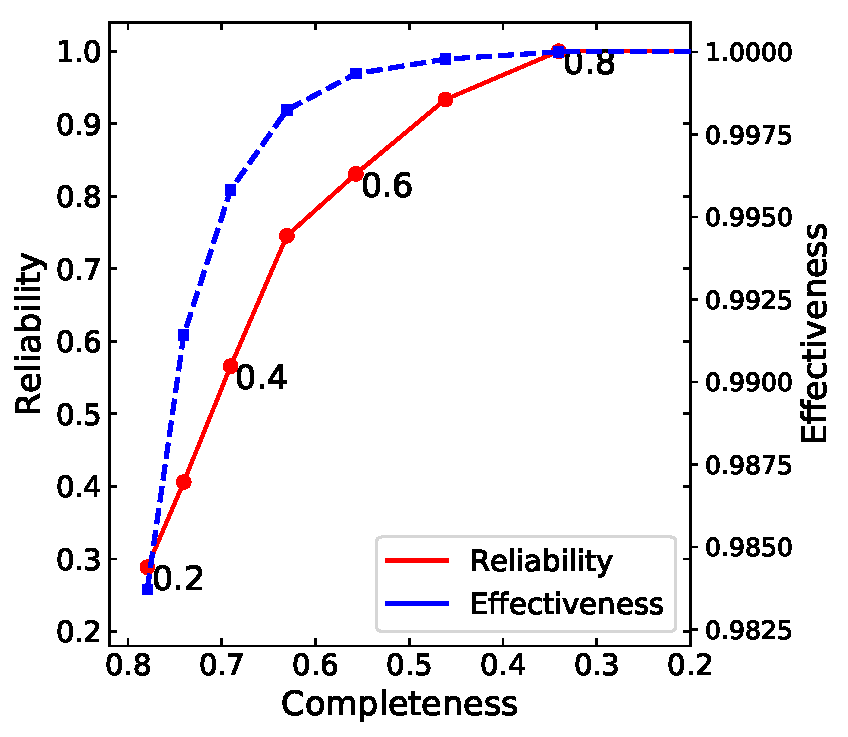
\includegraphics[width=.98\linewidth]{f13-top.pdf} \\
  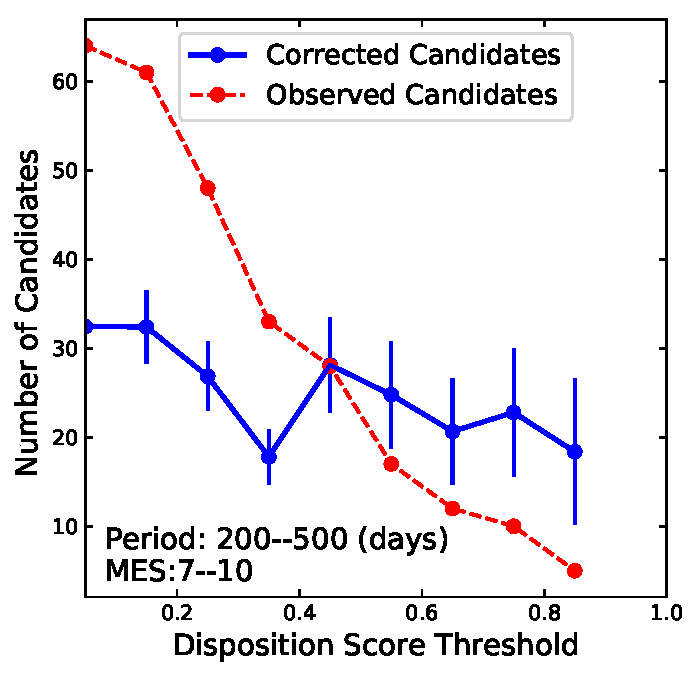
\includegraphics[width=.98\linewidth]{f13-bottom.pdf}
  \end{tabular}
  \caption{\label{f:adjscore}[Top] The reliability (red) and effectiveness (blue) of the DR25 catalog as a function of Completeness for MES~$\leq$~10 and periods between 200 and 500\,d PCs that result when using different disposition score thresholds (shown as black numbers) to select the PCs. Higher disposition score thresholds result in higher reliability but lower completeness. Note, the completeness axis increases to the left.  [Bottom] The number of PCs (in red) in the same period and MES space when making a cut on different disposition scores.  The blue line corrects the number of candidates for the completeness and reliability. The error bars only reflect a Poisson error based on the number of observed planet candidates shown in red.}
 \end{center}
 \end{figure}


